\section{Cloudsysteme --- Funktionalität}
\label{sec:cloudfunktionalitaet}

\paragraph{Was ändert sich in der Cloud?}
\begin{itemize}
	\item Physischer Entwurf muss automatisch erfolgen
	\item Obligatorische Datenverteilung
	\item Anfrageauswertung in Gegenwart anderer Anfragen
		\\*
		\( \leadsto \) entsprechende Planung
	\item Unterschiedliche QoS-Vereinbarungen mit unterschiedlichen Dienstnehmern
	\item Plötzliche extreme Zunahme von Zugriffen eines Dienstnehmers i.A. nicht vorhersehbar 
		\\*
		\( \leadsto \) Infrastruktur sollte damit umgehen können
	\item \emph{Secure Storage}: Verschlüsselung der Daten, trotzdem soll Dienstanbieter möglichst großen Teil der Anfrageauswertung übernehmen
\end{itemize}

\paragraph{Relationale Algebra}
\begin{itemize}
	\item \textbf{Projektion} $\pi$: Optimierung: bei vielen Projektionen hintereinander reicht die zuletzt ausgeführte auch allein:
		\\*
		\( \pi \)\lstinline{[KName](}\( \pi \)\lstinline{[KName, Land](Kuenstler))} \( \leadsto \) \( \pi \)\lstinline{[KName](Kuenstler)}
	\item \textbf{Selektion} $\sigma$: Optimierung: Selektionen lassen sich beliebig vertauschen, manchmal auch Projektion und Selektion
	\item \textbf{Verbund} $\bowtie$: Kommutativ, Assoziativ (Aber: Ausführungsreihenfolge kann erhebliche Performance-Unterschiede erzeugen)
		\\*
		\emph{Nested-Loop Join}: Teuer ($O(n * m)$), da pro Eintrag links über alle rechten Einträge iteriert wird. \\*
		Besser: \emph{Bock-Nested-Loop Join }(Arbeitsspeicher ausnutzen)
		\\*
		\emph{Merge Join}: Beide Relationen sortieren, dann Eintrag für Eintrag Merge-Technik anwenden (linear wenn X Schlüssel)
\end{itemize}

\paragraph{Logische vs. physische Operatoren}
\begin{itemize}
	\item DBS enthält meist mehrere pysische Operatoren und Implementierungen für den gleichen logsichen Operator
	\item DBS sucht selbst den optimalen pysischen Operator heraus
	\item Pysische Operatoren können dabei mehrere logische Operatoren zusammenfassen
\end{itemize}

\paragraph{Blockierende/Nichtblockierende Operatoren}
\begin{itemize}
	\item Operator blockiert \( \Leftrightarrow \) Ergebnis des Operators muss vor Ausführung des nachfolgenden vollständig berechnet sein \\* (z.B. Sort-Operator)
\end{itemize}

\paragraph{Histogramme}
\begin{itemize}
	\item Zeigt Auftrittshäufigkeit eines Intervalls (Bucket)
	\item \textbf{Equi-Width-Histogramm}: Breite aller Buckets gleich
	\item \textbf{Equi-Depth-Histogramm}: Auftrittshäufigkeit aller Buckets gleich
	\item Nützlich bei ein-Attribut-Anfragen, sonst nicht so:
		\\*
		Mehrdimensionale Histogramme schwer konstruierbar und wartbar, Anzahl Attributkombinationen exponentiell wachsend zur Anzahl der Attribute
\end{itemize}

\paragraph{Synchroner und asynchroner Zugriff}
\begin{itemize}
	\item \textbf{Synchron}: innerhalb einer Transaktion
	\item \textbf{Asynchron}: mehrere Transaktionen
\end{itemize}

\paragraph{Service-Level Agreements}
\begin{itemize}
	\item Vereinbarung zwischen Client und Server bzgl. Dienstausführung
		\\*
		``Antwort innserhalb von 300ms für 99,9\% der Aufrufe bei 500 Zugriffen pro Sekunde''
\end{itemize}

\paragraph{Quorum Consensus}
\begin{itemize}
	\item Szenario: Replikation mit \( n \) Knoten
		\\*
		\( \leadsto \) Wie strenge Konsistenz beim Schreiben sicherstellen? Was, wenn nicht alle Knoten verfügbar?
	\item Lesen: Lese Mindestanzahl von Versionen (\( R \)), nehme aktuelle
	\item Schreiben: Aktualisiere Mindestanzahl von Kopien (\( W \))
	\item Jede Kopie erhält Versionsnummer
	\item Üblich ist \( Q_R+Q_W > N \)
\end{itemize}



\paragraph{P2P}
\begin{itemize}
	\item \emph{peer to peer}-Systeme:
		\\*
		Jeder Knoten für Ausschnitt des Schlüsselraums verantwortlich
		\\*
		Verwaltung von (Schlüssel, Wert)-Paaren
		\\*
		(put, get)-Interface
		\\*
		Zu Größe des Schlüsselraums logarithmischer Suchaufwand
	\item Beispiel: \emph{Chord} \\*
		Zentrale Datenstruktur: \emph{identifier circle}, \emph{chord ring}\\*
		Schlüssel $k$ gehört zum im Uhrzeigersinn nächsten Knoten\\*
		Einfaches Hinzufügen / Entfernen von Knoten möglich
		\\* Suche: Jeder Knoten hat \emph{finger table}, \emph{i}-ter Eintrag von Knoten \( n \): successor(\( n+2^{i-1} \)) (\( m \) Anzahl Bits)
	\begin{figure}[H]\centering\label{Chord}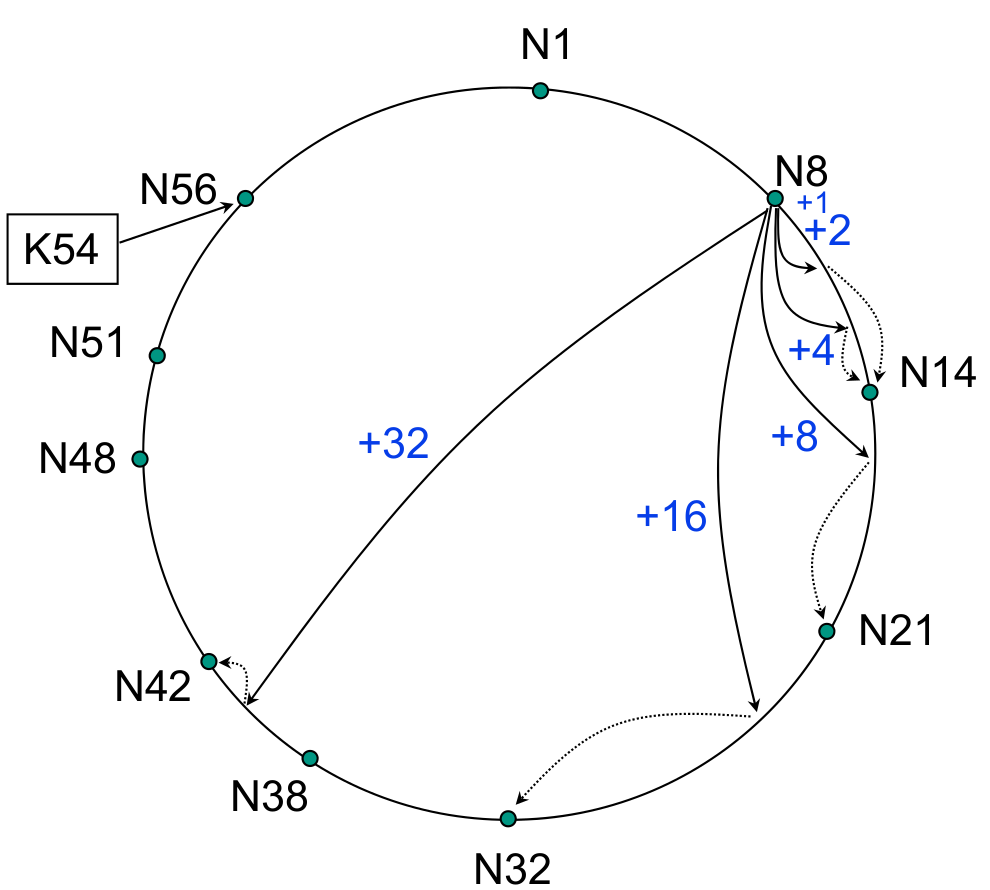
\includegraphics[width=.3\linewidth]{Chord}\end{figure}
	\item Replikation über \emph{chained replication}: Schlüssel nicht nur bei einem Knoten, sondern auch bei \( k \) Nachfolgern einfügen
	\item \textbf{Heterogenität}: Knoten können unterschiedlich leistungsstark sein (ggf. unterschiedliche Zuständigkeitsbereiche, unterschiedliche Last)
	\item Umrechnen von Anwendungs- in Systemschlüssel, um Last zu verteilen (gleich / ungleich, evtl. auf mehrere Positionen)
\end{itemize}

\paragraph{Dynamo}
\begin{itemize}
	\item Key-Value-Store
	\item get-/put-Interface
	\item Objekte BLOBs \( \leadsto \) kein DB-Schema \( \leadsto \) Interpretieren nötig
	\item Keine Isolation \( \leadsto \) keine totale Konsistenz
	\item Schreibzugriff jeweils nur für ein Objekt
\end{itemize}
\begin{figure}[H]\centering\label{UebersichtDynamo}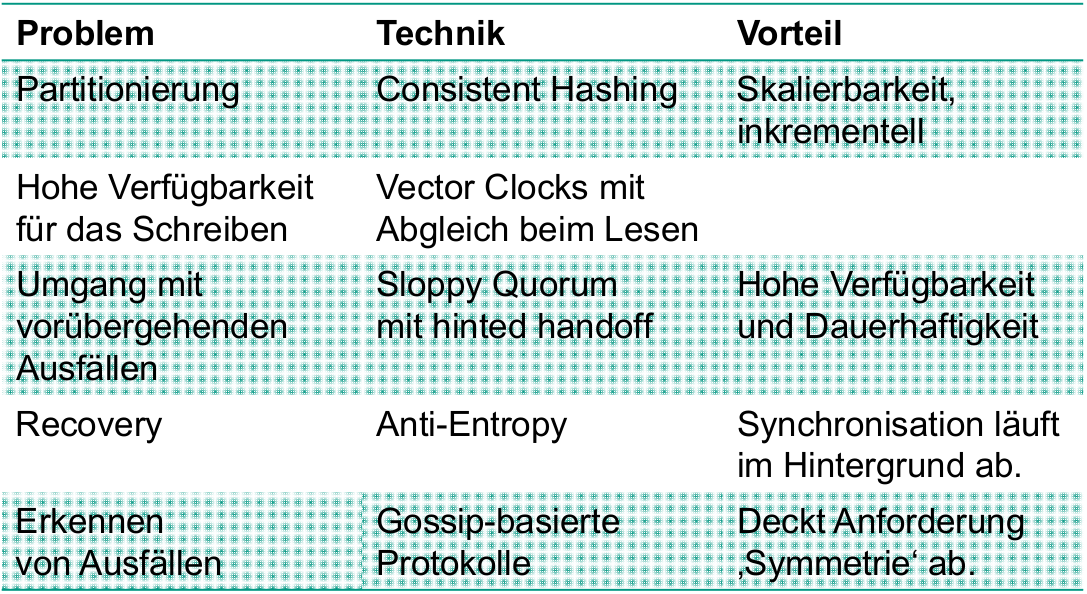
\includegraphics[width=0.33\textwidth]{UebersichtDynamo}\end{figure}

\paragraph{Dynamo --- Vector Clocks}
\begin{itemize}
	\item Ziel: eventual consistency
	\item Liste von (Knoten, Zähler)-Paaren (eine Liste pro Version) \( \leadsto \) Erfassung der Zusammenhönge zwischen Versionen
	\item Quorum-basierte Techniken \( \leadsto \) Inkonsistenzen vermeiden
	\item Vector-Clock-basierte Techniken \( \leadsto \) Inkonsistenzen erkennen und auflösen
	\item Unterschiedliche Knoten können Schreiboperationen absetzen \\* \( \leadsto \) Eine Liste von (Knote, Zähler)-Paaren pro Version
	\item Version 1 ist Vorgänger von Version 2, wenn jeder Zähler in Liste von V1 einen kleineren Wert hat als in der von V2
	\item Update (put) muss festlegen, welche Version aktualisiert werden soll
	\item Get gibt i.A. mehrere Versionen zurück
	\item Kombination mit \emph{Sloppy Quorum}: \( Q_R+Q_W < N \)
\end{itemize}



\paragraph{Datenbanktechnologie auf Dynamo}
\begin{itemize}
	\item Dynamo kein DBS im klassischen Sinn: Niedrigere Schnittstelle für Anwendungsentwicklung
	\item Aber: Bessere nichtfunktionale Eigenschaften
	\item Im Folgenden: Ansätze für DBS 'On Top of' Dynamo
\end{itemize}

\paragraph{Scale Independence}
\begin{itemize}
	\item Anfrage ist \emph{scale-independent}
		\\*
		\( \leadsto \) Laufzeitverhalten unabhängig von DB-Größe
	\item Anfragenklassifikation nach Aufwand: \\*
		- Klasse I (konstant):
			\\*
			z.B. Schlüssel-Zugriff, \lstinline[language=sql]{LIMIT}-beschränkt, Paginierung\\*
			Join auf Fremdschlüssel \\*
		- Klasse II (beschränkt):
			\\*
			Explizite Begrenzung liegt vor
			\\*
			Als Kardinalität im erweiterten DB-Schema darstellbar \\*
		- Klasse III (linear / sublinear):
			\\*
			z.B. Ausgabe aller Kunden/Produkte
		\item Klasse IV (superlinear):
			\\*
			z.B. Clustering-Algo, der Self-Join der zugrundeliegenden Relation ausführt
	\item \( \leadsto \) \emph{PIQL} (\emph{performance insightful query language}) - Scale Independent durch Erweiterungen und Beschränkungen der Anfragesprache
\end{itemize}

\paragraph{Physische Optimierung}
\begin{itemize}
	\item Zwei Arten von physischen Operatoren: \\*
		1. \emph{remote operator}: Zugriffe auf key-value store und elementare Verarbeitungsschritte \\*
		2. Client-seitige Operatoren für Query-Logik
	\item Remote Operator: Muss explizite Beschränkung der Größe (und damit der Ausführungsdauer) des Zwischenergebnisses enthalten (i.A. \lstinline{dataStop}-Operator; Fehlermeldung und Nichtausführung wenn dies nicht der Fall ist)
	\item Remote-Operatoren: \\*
		- \emph{IndexScan}: Prädikat muss zusammenhängendem Ausschnitt des indexierten Wertebereichs entsprechen,\\*
		``Sort'' muss Sortierreihenfolge des Index sein \\*
		- \emph{IndexForeignKeyJoin}: Beschränkung durch Fremdschlüsseleigenschaft \( \leadsto \) kein logischer Stop-Operator, linker Teilausdruck enthält Fremdschlüssel \\*
		- \emph{SortedIndexJoin}: Bei Sortierung des Inputs nach Join Key lässt sich aus limit hint-Begrenzuung der Anzahl an Datenobjekten pro Schlüssel ableiten
\end{itemize}

\paragraph{SLO Compliance-Vorhersage}
\begin{itemize}
	\item SLO = \emph{serivce-level objectives}
	\item Größenbeschränkung Zwischenergebnisse noch keine Garantie für insgesamt beschränkten Aufwand
	\item Wenn anliegende Last sehr groß kann IndexScan-Ausführung beliebig lange dauern
	\item Histogramm-Lookup über Zufallsverteilung (Tupelgröße, Anzahl erwarteter Tupel)
\end{itemize}

\begin{fragen}
	\item Was für Möglichkeiten kennen Sie, den Join zu implementieren? Weche Komplexität haben sie?
	\item Welche Möglichkeiten kennen Sie, den Aufwand, den eine Anfrage verursacht, zu reduzieren/begrenzen?
\end{fragen}